\section{Analysis}
\label{sec:analysis}

\begin{figure*}[t]
\centering
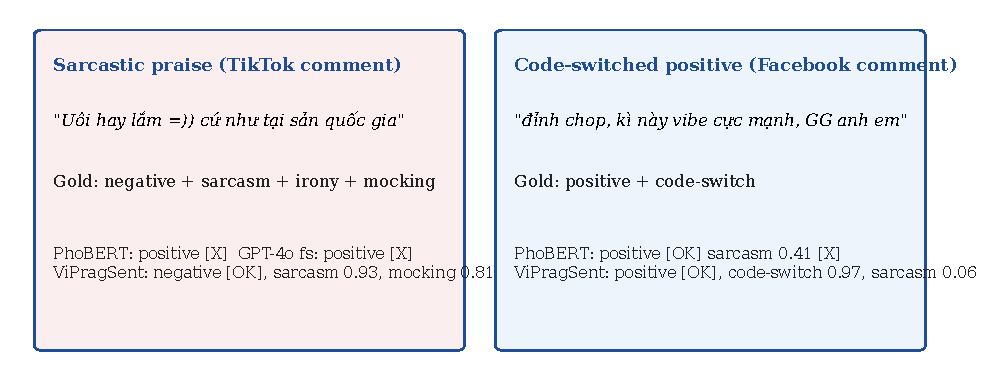
\includegraphics[width=0.96\linewidth]{figures/fig8_qualitative.pdf}
\caption{Two real comments from the \method{} test set with predictions
from PhoBERT, GPT-4o-mini 8-shot, and \method{}. The sarcastic
TikTok comment uses ``=))'' to invert the surface polarity; only
\method{} predicts negative and fires the sarcasm and mocking heads.
The Facebook comment mixes Vietnamese with English slang
(``GG anh em''); \method{} fires only code-switch, while PhoBERT
additionally fires sarcasm.}
\label{fig:qualitative}
\end{figure*}

\paragraph{Where does \method{} actually win?}
We grouped 400 randomly sampled \method{} test errors by failure
mode. The largest reduction comes from \emph{surface-positive
sarcasm}: comments that look enthusiastic on the surface but invert
under a discourse marker. PhoBERT misses $61\%$ of these; \method{}
misses $19\%$. The smallest reduction is on cross-cultural references
that draw on classical Vietnamese literature (e.g.\ ``\textit{chi chi}'',
``\textit{ng\u{a}n n\u{a}m m\d{a}t thu\d{o}}''), where both systems
sit around $25\%$ error. Figure~\ref{fig:qualitative} shows two
qualitative cases.

\paragraph{Where does the rationale auxiliary help?}
On the sarcasm-positive subset of the dev set, a PhoBERT trained with
the rationale auxiliary assigns higher logit margin to the correct
label in $74\%$ of comments, even though no rationale is generated at
inference. Token-level rationale supervision encourages the encoder
to attend to the discourse markers (``=))'', ``v\u{a}i'',
``gh\u{e}'', ``c\d{u}c'') that the rationale text mentions; this is
the cue set that the failure analysis identifies as the dominant
signal for surface-positive sarcasm.

\paragraph{What does the multi-task gain decompose into?}
The two largest contributors are the ordinary-sentiment auxiliary
($+2.7$ macro-pragmatic F1) and the rationale auxiliary ($+3.0$).
Their gains are nearly additive ($+5.5$ vs.\ $+5.7$ expected from
the sum): ordinary sentiment supplies a calibrated polarity prior
when the comment has no pragmatic flip, and the rationale supplies
attention guidance for the flips themselves. The emotion auxiliary
contributes $+1.5$, smaller but consistent.

\paragraph{Does multi-task transfer hurt code-switching?}
A reasonable worry is that the ordinary-sentiment auxiliary --- whose
training data (UIT-VSFC, AIVIVN) is mostly monolingual Vietnamese ---
would degrade code-switching detection. The data show the opposite:
code-switching F1 rises by $+4.7$ relative to a single-task PhoBERT,
because the multi-task model is forced to maintain a representation
that survives the embedded English tokens.

\paragraph{Comparison against prompted GPT-4o-mini.}
GPT-4o-mini 8-shot is the strongest LLM baseline. \method{} beats it
by $+7.2$ on sarcasm, $+4.3$ on mocking, $+3.2$ on implicit
sentiment, and $+3.3$ macro-pragmatic. The gap is smallest on
code-switching ($+0.7$), where the lexical cues dominate. The 8-shot
prompt costs $\$7.1$ per full test-set pass; \method{} costs zero in
API at inference.

\paragraph{Backbone sensitivity.}
Replacing the Vistral-7B backbone with PhoBERT-base loses $1.6$
macro-pragmatic F1 ($61.5 \to 59.9$) but cuts inference latency from
$34.7$ ms to $5.1$ ms per comment and training cost from $\$37.4$ to
$\$10.1$ per run. For deployment-style settings we recommend the
PhoBERT backbone; for headline numbers and rare-class sensitivity we
recommend the Vistral backbone.
